\section{Pre-pilot descriptive diagnostics (2000--2006)}
\label{sec:diagnostics}

Three descriptive studies were run on the earliest years of the sample before any model was scored. They
test the premises of the design (the horizon, regime dependence of the cross-section, industry regimes)
on data the pilot and the test period never use.

\begin{keybox}{Rules that applied to all three}
\begin{itemize}
\item \textbf{Hard date guard 2000-01-01 to 2006-12-31.} Forward windows end by 2006-12-31, so the last scored
  date moves back by $h$; no 2007 return was read. The pilot's validation years (2007--2009) and the test
  period (2010--2024) are untouched.
\item \textbf{Descriptive only.} No result feeds back into a design choice: not the horizon (unless the evidence
  overturned it), not $K$ (Q18), not the features (Q26), not the industry-gate form (Q28).
\item \textbf{Readings written down before each run}, including what a negative result would mean.
\item Code written and tested on synthetic data by Claude Code (briefs 10 C and 11); real runs by Tom.
\end{itemize}
\end{keybox}

\begin{whybox}[Why run diagnostics before the pilot]
The thesis rests on two premises: that a five-day horizon is the right place to look, and that the cross-section
of returns depends on the market's regime. Both can be checked cheaply on years that play no other role. Running
them first means a failed premise is discovered before compute is spent, and a confirmed one enters the thesis
as evidence fixed in advance rather than as a story told after the results.
\end{whybox}

\subsection{The IC decay curve: is five days the right horizon?}

\paragraph{Method (brief 10 C).} For 16 signals (the two reversal and two momentum characteristics of the JKP
block and the 12 short-horizon characteristics), the daily cross-sectional rank IC against the market-neutral
forward return at $h = 1, 2, 3, 5, 10$, averaged over 2000--2006, with Hansen--Hodrick t-statistics at lag $h-1$.

\paragraph{How to read it.} If a signal predicts every day of the next $h$ equally, its IC grows like $\sqrt h$
(a factor 2.2 at $h=5$, 3.2 at $h=10$) and its overlap-corrected t-statistic stays roughly flat. If it predicts
only the next day, its IC shrinks like $1/\sqrt h$ and its t-statistic falls. So a falling t-statistic means the
signal's information is fading.

\begin{center}
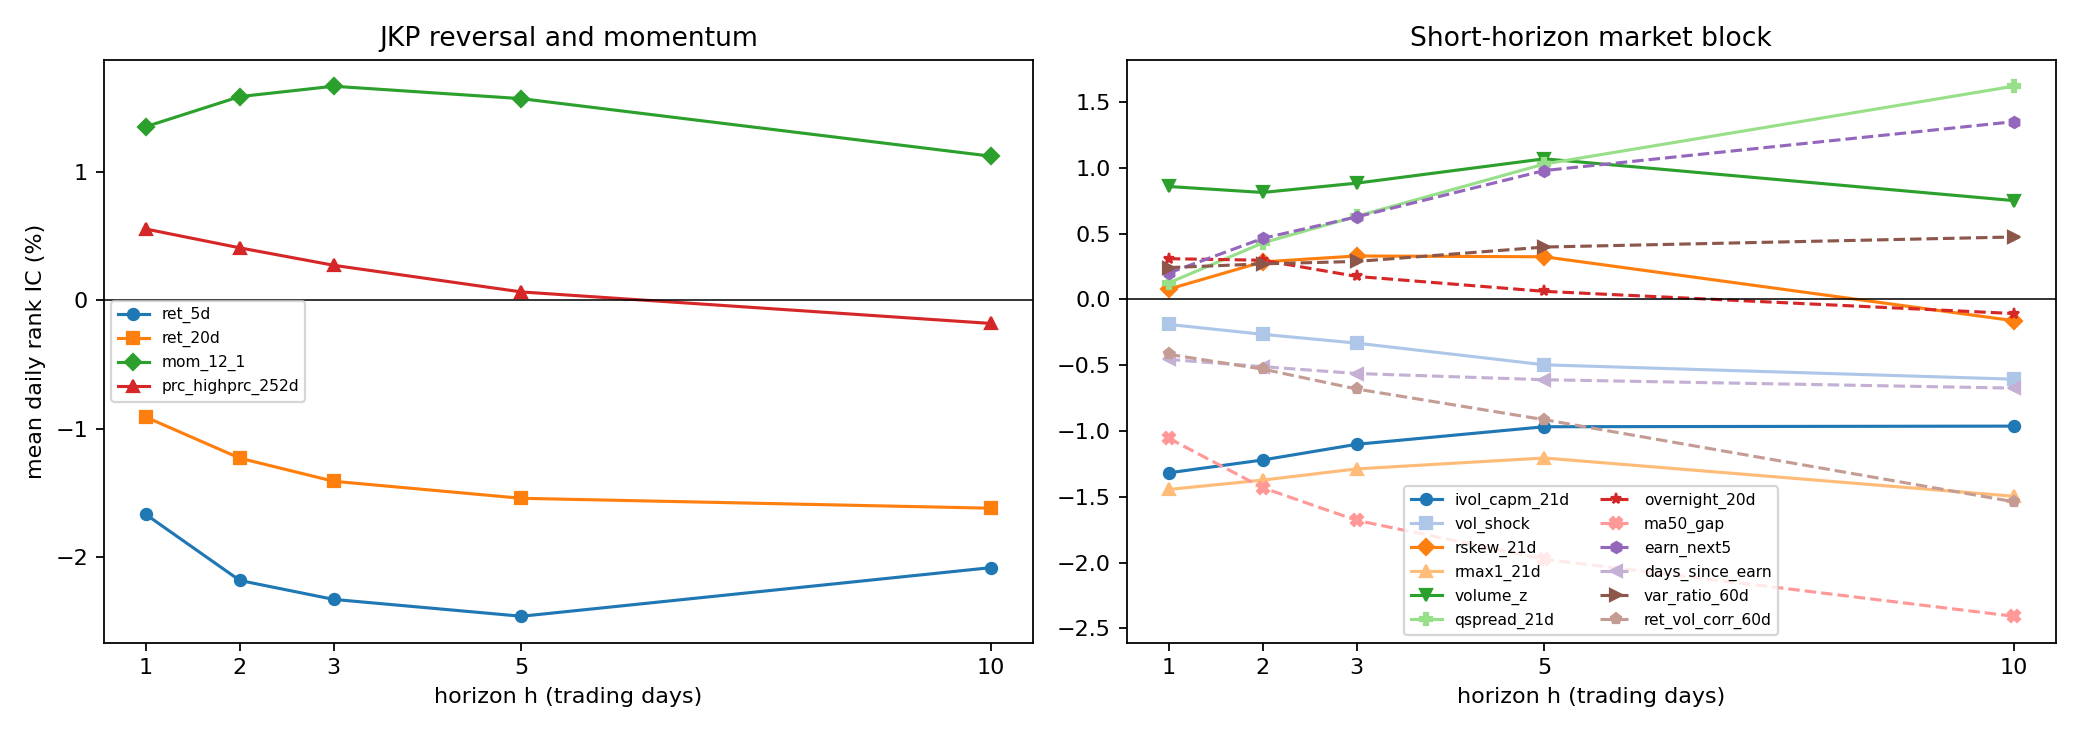
\includegraphics[width=\textwidth]{fig/ic_decay_redrawn.png}
\end{center}

{\small
\begin{tabular}{@{}lrrrrl@{}}
\toprule
Signal & IC $h{=}1$ & IC $h{=}5$ & IC $h{=}10$ & $t$ ($h{=}5$) & Shape\\
\midrule
\texttt{ret\_5d} (one-week reversal) & $-1.67$ & $-2.46$ & $-2.08$ & $-4.21$ & builds to 5, then done\\
\texttt{volume\_z} (abnormal volume) & $+0.86$ & $+1.07$ & $+0.75$ & $4.05$ & peaks at 5, most robust\\
\texttt{mom\_12\_1} (momentum) & $+1.36$ & $+1.57$ & $+1.12$ & $1.43$ & peaks at 3, fades\\
\texttt{ivol\_capm\_21d} & $-1.32$ & $-0.97$ & $-0.96$ & $-0.90$ & strongest next day\\
\texttt{rmax1\_21d} (max return) & $-1.44$ & $-1.20$ & $-1.50$ & $-1.14$ & flat IC, $t$ falls\\
\texttt{ret\_20d} (one-month reversal) & $-0.91$ & $-1.54$ & $-1.62$ & $-1.97$ & still building\\
\texttt{ma50\_gap} & $-1.06$ & $-1.97$ & $-2.41$ & $-2.33$ & slow, close to $\sqrt h$\\
\texttt{ret\_vol\_corr\_60d} & $-0.42$ & $-0.91$ & $-1.54$ & $-1.92$ & slow\\
\texttt{qspread\_21d} (spread) & $+0.13$ & $+1.03$ & $+1.62$ & $1.80$ & nothing next day, accrues\\
\texttt{earn\_next5} & $+0.20$ & $+0.98$ & $+1.35$ & $3.25$ & the event falls in the window\\
\texttt{days\_since\_earn} & $-0.46$ & $-0.61$ & $-0.67$ & $-1.51$ & weak\\
\texttt{prc\_highprc\_252d} & $+0.56$ & $+0.07$ & $-0.18$ & $0.06$ & gone by 5\\
\bottomrule
\end{tabular}}

ICs in percent. Volatility shock, realised skewness, overnight return and variance ratio have $|t| < 1.3$ at every
horizon.

\paragraph{Findings.}
\begin{itemize}
\item \textbf{The strongest signal peaks at $h=5$.} One-week reversal builds to five days and adds nothing after;
  abnormal volume also peaks at five.
\item \textbf{Fast signals} (idiosyncratic volatility, maximum return, momentum, the 52-week high) lose IC and
  t-statistic by five days: most of their information is in the first two or three days.
\item \textbf{Slow signals} (distance from the 50-day average, the spread, the earnings dummy, one-month reversal)
  keep building to ten days; a one-day target would miss them.
\item \textbf{Nothing points to three days beating five.}
\end{itemize}

\paragraph{Caveats.} 80 tests (16 signals $\times$ 5 horizons): under Bonferroni ($|t|>3.4$) only one-week reversal
and abnormal volume ($h\le5$) and the earnings dummy ($h=10$) clear the bar. Regimes are pooled: 2000--2006 mixes the
2000--02 bear market with the calm of 2003--06, so a signal with opposite signs in calm and stress averages to near
zero (the motivation for the next study).

\begin{decbox}{Decided 2026-10-09 (Q21 follow-up)}
$h = 5$ confirmed; the horizon question is closed. The Q26 inputs are unchanged.
\end{decbox}

\begin{whybox}[Why the weak signals were not dropped]
The feature list was fixed by a rule (two representatives per theme) precisely so that it would not be chosen on
outcomes. Pruning signals for weak pooled ICs would turn a rule-based selection into an outcome-based one, even on
pre-pilot years. And a pooled IC near zero is exactly what a signal whose sign depends on the regime would show,
which is a reason for a regime gate, not against the signal.
\end{whybox}

\subsection{Market regimes on 2000--2006}

\paragraph{Method (brief 11 A).} The Hamilton gate fitted on the CRSP S\&P 500 index's daily log return over
2000--2006 with equal weights (the pilot had not yet chosen the memory), $K=2$ as the main case and $K=3$ as a check;
only filtered probabilities; for each horizon the window-average gate weight of Q27. The parameters are estimated on
the whole span, so the probabilities are causal in the data but not in the parameters: an in-sample description,
not a forecast. A parameter-free check: ``stress'' when the trailing 20-day market volatility is above its 2000--2006
median.

\begin{center}
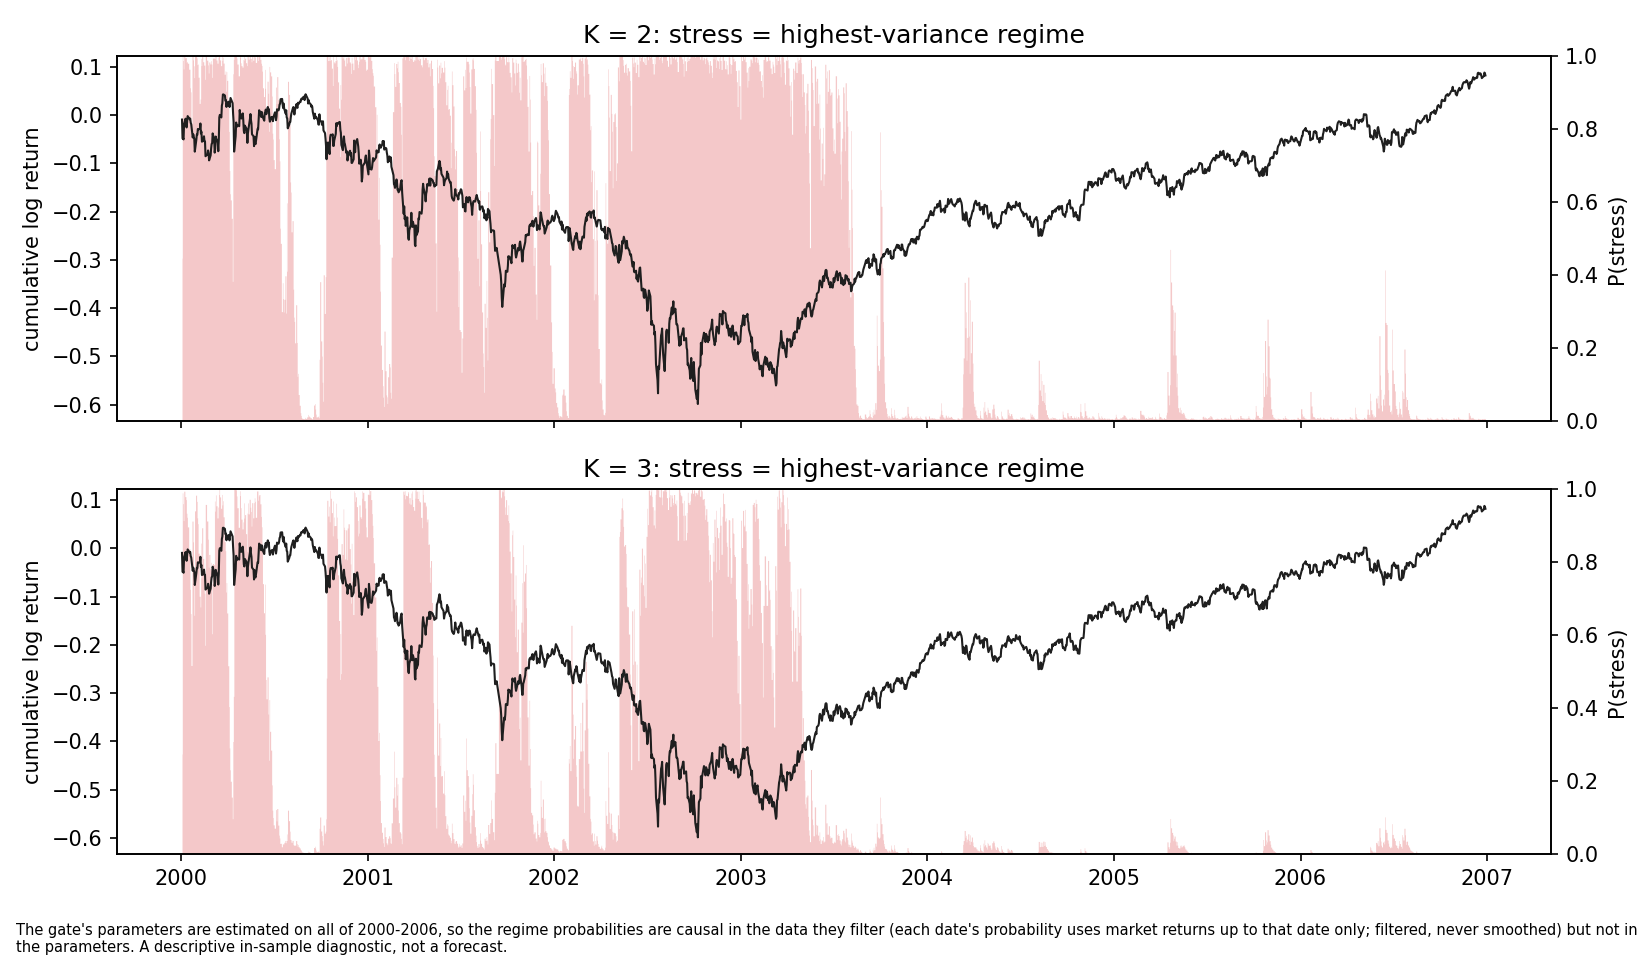
\includegraphics[width=0.92\textwidth]{fig/market_regimes_2000_2006.png}
\end{center}

\begin{itemize}
\item \textbf{$K=2$: one long stress block}, January 2000 to August 2003, calm afterwards. Daily volatility 0.69\% calm
  against 1.53\% stress; expected durations 229 and 177 days; all 24 starting points converged to the same optimum.
\item \textbf{$K=3$}: volatilities 0.60\%, 0.98\% and 1.75\%, expected durations 110, 46 and 79 days, so the stress state
  breaks into episodes inside 2000--03.
\end{itemize}

\begin{warnbox}{What this means for the next study}
With $K=2$ the regime contrast is largely ``2000--03 against 2003--06''. Any slow change in how a signal worked over
those years lands inside the ``regime'' contrast. This is the slow-drift case of the synthetic size check, where both
t-statistics over-reject. The trailing-volatility split switches far more often and is less tied to the 2003 break,
which is why it is the key robustness check below.
\end{warnbox}

\subsection{The IC split by regime}

\paragraph{Method (brief 11 B).} 18 signals (the 16 above plus within-industry reversal and industry momentum) at
$h=1$--$10$. For each date the gate gives regime weights $w_k(t)$ summing to one. Two estimates per regime:
\begin{itemize}
\item a \textbf{weighted mean IC}, $\sum_t w_k(t)\,\mathrm{IC}_t / \sum_t w_k(t)$, with its effective number of dates;
\item a \textbf{pure-regime IC} $c_k$ from the regression without intercept
  \[\mathrm{IC}_t=\sum_k c_k\,w_k(t)+e_t,\]
  the IC on a day fully in regime $k$. The \textbf{contrast} is $c_{\text{stress}}-c_{\text{calm}}$, with sandwich
  standard errors under two HAC choices: Hansen--Hodrick at lag $h-1$ and Newey--West at lag $\max(h-1,20)$, the
  second because a persistent regime probability makes residuals correlated beyond the target overlap.
\end{itemize}
Robustness: filtered instead of window weights, a hard split (weight above 0.5), and the trailing-volatility state.

\paragraph{Pre-specified tests.} Fixed before the run from the literature, at $K=2$, $h=5$, Hansen--Hodrick, one-sided,
with a Holm correction across the five:
\begin{itemize}
\item \textbf{H1} reversal is stronger in stress, for one-week, one-month and within-industry reversal (Nagel 2012;
  Hameed \& Mian 2015);
\item \textbf{H2} momentum is weaker in stress, for stock and industry momentum (Cooper, Gutierrez \& Hameed 2004;
  Wang \& Xu 2015; Daniel \& Moskowitz 2016).
\end{itemize}
Everything else is an exploratory family with Benjamini--Hochberg q-values.

\paragraph{Results: the five primary tests ($K=2$, $h=5$, window weights).}\mbox{}\par\smallskip

\begin{center}{\small
\begin{tabular}{@{}lrrrrr@{}}
\toprule
Signal & IC calm & IC stress & Contrast & $t$ (HH) & Holm $p$\\
\midrule
\texttt{ret\_5d} & $-1.70$ & $-3.46$ & $-1.76$ & $-1.31$ & 0.38\\
\texttt{ret\_20d} & $+0.20$ & $-3.83$ & $-4.03$ & $-2.17$ & 0.076\\
\texttt{ret\_20d\_ind\_rel} & $-0.74$ & $-2.19$ & $-1.45$ & $-1.11$ & 0.40\\
\texttt{mom\_12\_1} & $+2.83$ & $-0.07$ & $-2.90$ & $-1.10$ & 0.40\\
\texttt{ind\_mom\_12\_1} & $+0.58$ & $+0.74$ & $+0.17$ & $0.07$ & 0.53\\
\bottomrule
\end{tabular}}\end{center}
ICs and contrasts in percent.

\paragraph{Robustness of the contrasts (t-statistics, $h=5$).}\mbox{}\par\smallskip

\begin{center}{\small
\begin{tabular}{@{}lrrrrr@{}}
\toprule
Signal & $K{=}2$ HH & $K{=}2$ NW & $K{=}2$ hard & $K{=}3$ HH & Volatility split\\
\midrule
\texttt{ret\_5d} & $-1.31$ & $-1.43$ & $-1.28$ & $-1.43$ & $-0.68$\\
\texttt{ret\_20d} & $-2.17$ & $-2.42$ & $-1.89$ & $-3.05$ & $-2.16$\\
\texttt{ret\_20d\_ind\_rel} & $-1.11$ & $-1.24$ & $-0.83$ & $-1.78$ & $-1.27$\\
\texttt{mom\_12\_1} & $-1.10$ & $-1.13$ & $-1.17$ & $-1.23$ & $-0.96$\\
\texttt{ind\_mom\_12\_1} & $0.07$ & $0.08$ & $0.12$ & $-0.41$ & $0.43$\\
\bottomrule
\end{tabular}}\end{center}

\begin{center}
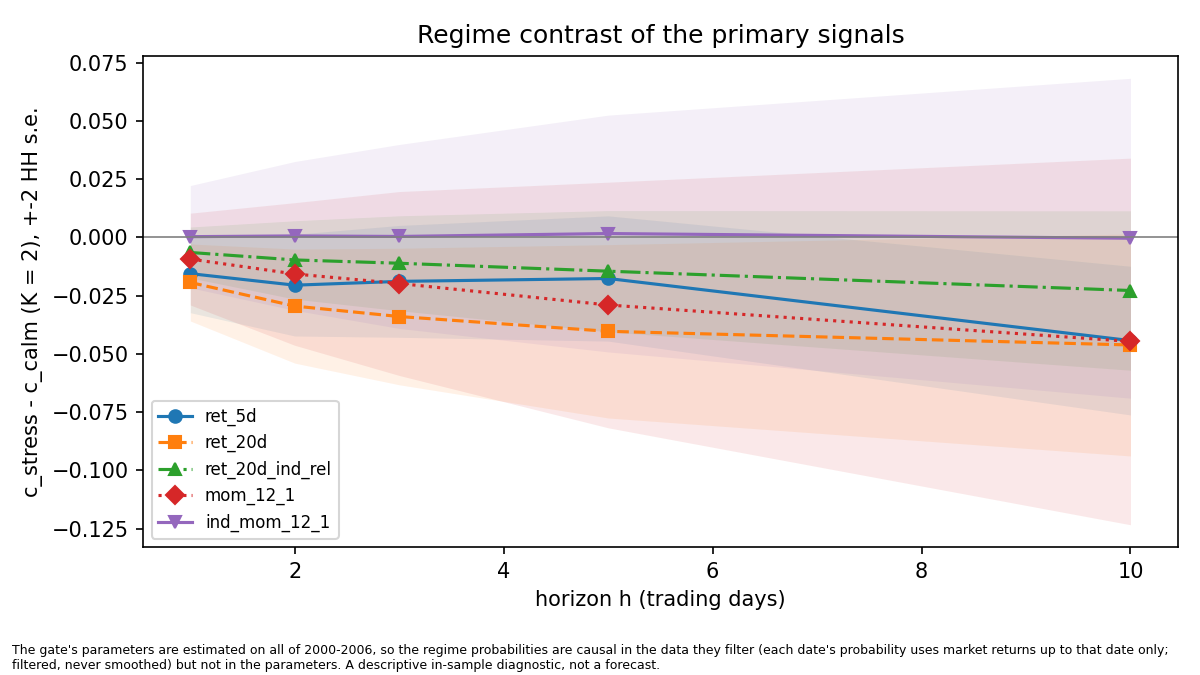
\includegraphics[width=0.78\textwidth]{fig/ic_regime_contrast_2000_2006.png}
\end{center}

\paragraph{Findings.}
\begin{itemize}
\item \textbf{The pattern matches the literature but is underpowered.} Four of five contrasts have the expected sign:
  one-week reversal is about twice as strong in stress, one-month reversal exists \emph{only} in stress, momentum
  works in calm and disappears in stress; industry momentum does not move. None survives Holm (smallest adjusted
  $p$ 0.076).
\item \textbf{One-month reversal is not just the 2003 break}: it keeps its contrast under the trailing-volatility
  split ($t=-2.16$) and is stronger at $K=3$ ($t=-3.05$). One-week reversal's contrast weakens under the volatility
  split ($-0.68$), so part of it may be drift.
\item \textbf{Exploratory family}: 11 of 175 contrasts reach $q<0.10$, none $q<0.05$. They are mainly abnormal volume
  (a stronger signal in stress at $h=3$--10, both $K$) and one-month reversal at $K=3$. These are hypotheses for
  2007--2024, not findings.
\end{itemize}

\begin{decbox}{Reading, by the rule written before the run: neutral}
Contrasts of the expected sign but not significant after Holm: consistent with the literature and with the
thesis's premise, but underpowered, because 2000--2006 contains essentially one long stress episode. The design is
unchanged. Regime dependence is tested properly where it matters: across the six stress episodes of 2010--2024 and
the 2008 crisis in the pilot years.
\end{decbox}

\subsection{Do sectors have their own regimes? (input to Q28)}

\paragraph{Method (brief 11 C).} For each GICS sector, the value-weighted daily return of its S\&P 500 members, as a
log return, both raw and \textbf{sector-relative} (sector minus index). A two-state Hamilton gate per sector and
series on 2000--2006, filtered probabilities. Measures: the share of days a sector is stressed while the market is
calm, the conditional probability of sector stress given market calm, the correlation of each sector's stress
probability with the market's, durations and episodes. Pre-written expectation: raw sector regimes largely copy the
market's; sector-relative ones should not.

\begin{center}
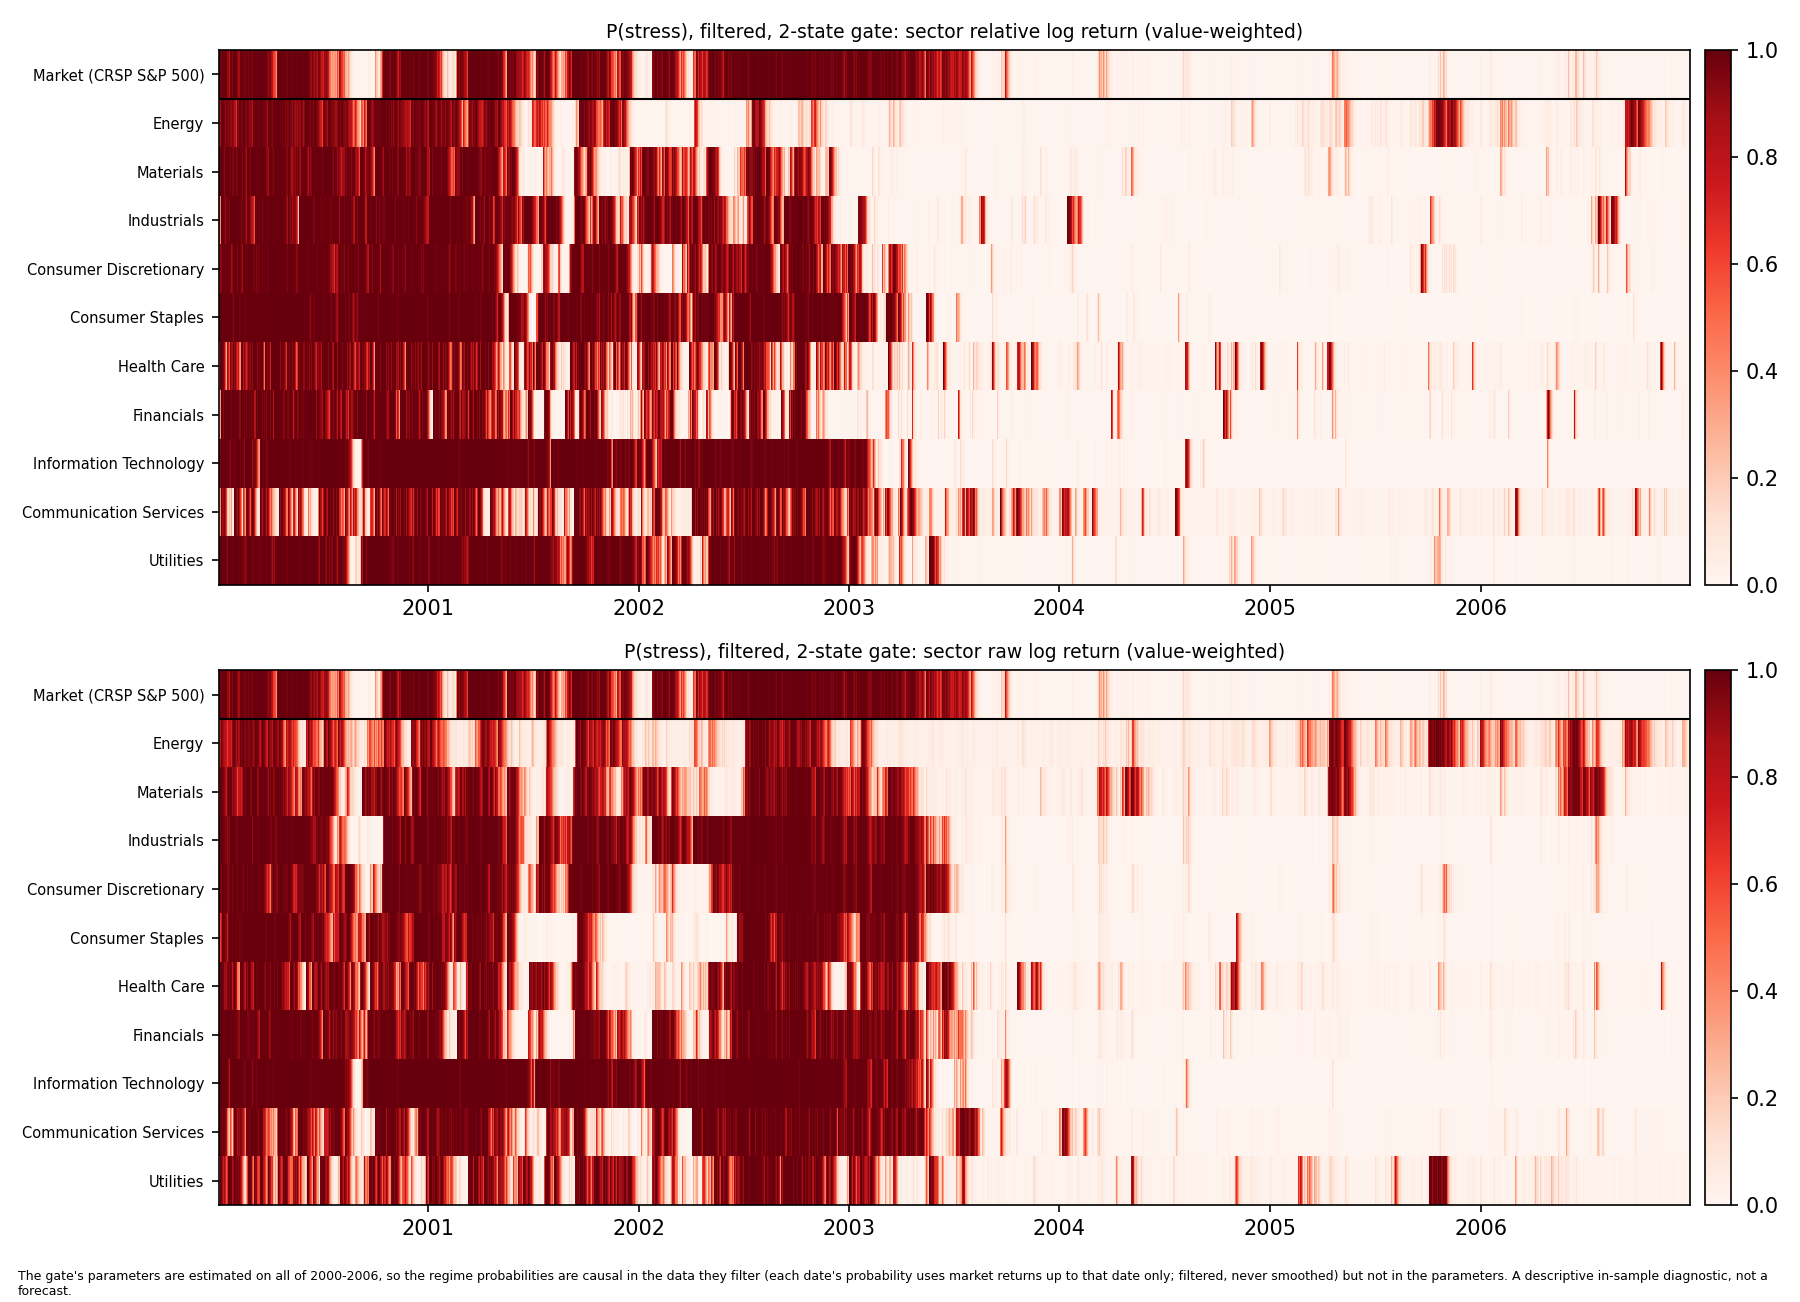
\includegraphics[width=\textwidth]{fig/sector_regimes_2000_2006.png}
\end{center}

\begin{center}\resizebox{\textwidth}{!}{%
\begin{tabular}{@{}lrrrrr@{}}
\toprule
Sector (relative, value-weighted) & Stressed & Stressed, market calm & P(stress $\mid$ calm) & Corr.\ with market & Episodes\\
\midrule
Energy & 28\% & 7.7\% & 13.7\% & 0.42 & 12\\
Materials & 30\% & 6.1\% & 10.8\% & 0.56 & 17\\
Industrials & 40\% & 9.3\% & 16.4\% & 0.61 & 16\\
Consumer Discretionary & 37\% & 5.8\% & 10.3\% & 0.70 & 13\\
Consumer Staples & 44\% & 7.0\% & 12.4\% & 0.80 & 11\\
Health Care & 37\% & 8.4\% & 14.8\% & 0.60 & 33\\
Financials & 30\% & 5.9\% & 10.5\% & 0.55 & 22\\
Information Technology & 44\% & 7.3\% & 13.0\% & 0.77 & 7\\
Communication Services & 35\% & 6.5\% & 11.5\% & 0.66 & 34\\
Utilities & 41\% & 6.4\% & 11.3\% & 0.77 & 9\\
\bottomrule
\end{tabular}}\end{center}

Real Estate has no names before 2016 (it was part of Financials) and was not fitted. Communication Services is the
thinnest sector (median 12 names, minimum 8).

\paragraph{Findings: between the two pre-written outcomes.}
\begin{itemize}
\item \textbf{Relative regimes follow the market less than raw ones, but still substantially}: median correlation with
  the market's stress probability 0.64 for relative series against 0.76 for raw. In the heat strips, relative stress
  mostly marks 2000--03, when sector returns diverged widely.
\item \textbf{Sector-own stress exists but is concentrated}: a sector is stressed while the market is calm on 6--9\% of
  days (conditional probability 10--16\%). The clearest sector-own episode is Energy in 2005--06, with sporadic
  Health Care and Communication Services spikes.
\item \textbf{Caveat}: the index contains the sector, so ``sector minus index'' partly cancels the largest sectors
  (technology was a fifth to a third of the index in 2000). A sector-minus-rest-of-market series would remove this.
\end{itemize}

\begin{openbox}{What this does and does not settle for Q28}
It informs the sub-questions on what the industry chain is fitted on (relative series are less market-driven but
need the cancellation fixed), granularity (thin sectors), and the descriptive check itself. It does \emph{not} choose
the form of the industry-level gate, which stays open; the 2000--2006 window has one market stress block, so the
co-movement of sector and market regimes may look different over 2007--2024.
\end{openbox}
